\interlude[0]{The Design of Rosenpass \\ \vspace{0.8em} \small and how to build post-quantum protocols}
\section{The Design of Rosenpass}

\begin{frame}[light]{}
  \vspace{1cm}
  \large
  \vollkorn

  \begin{columns}[c]
    \begin{column}{.30\linewidth}
      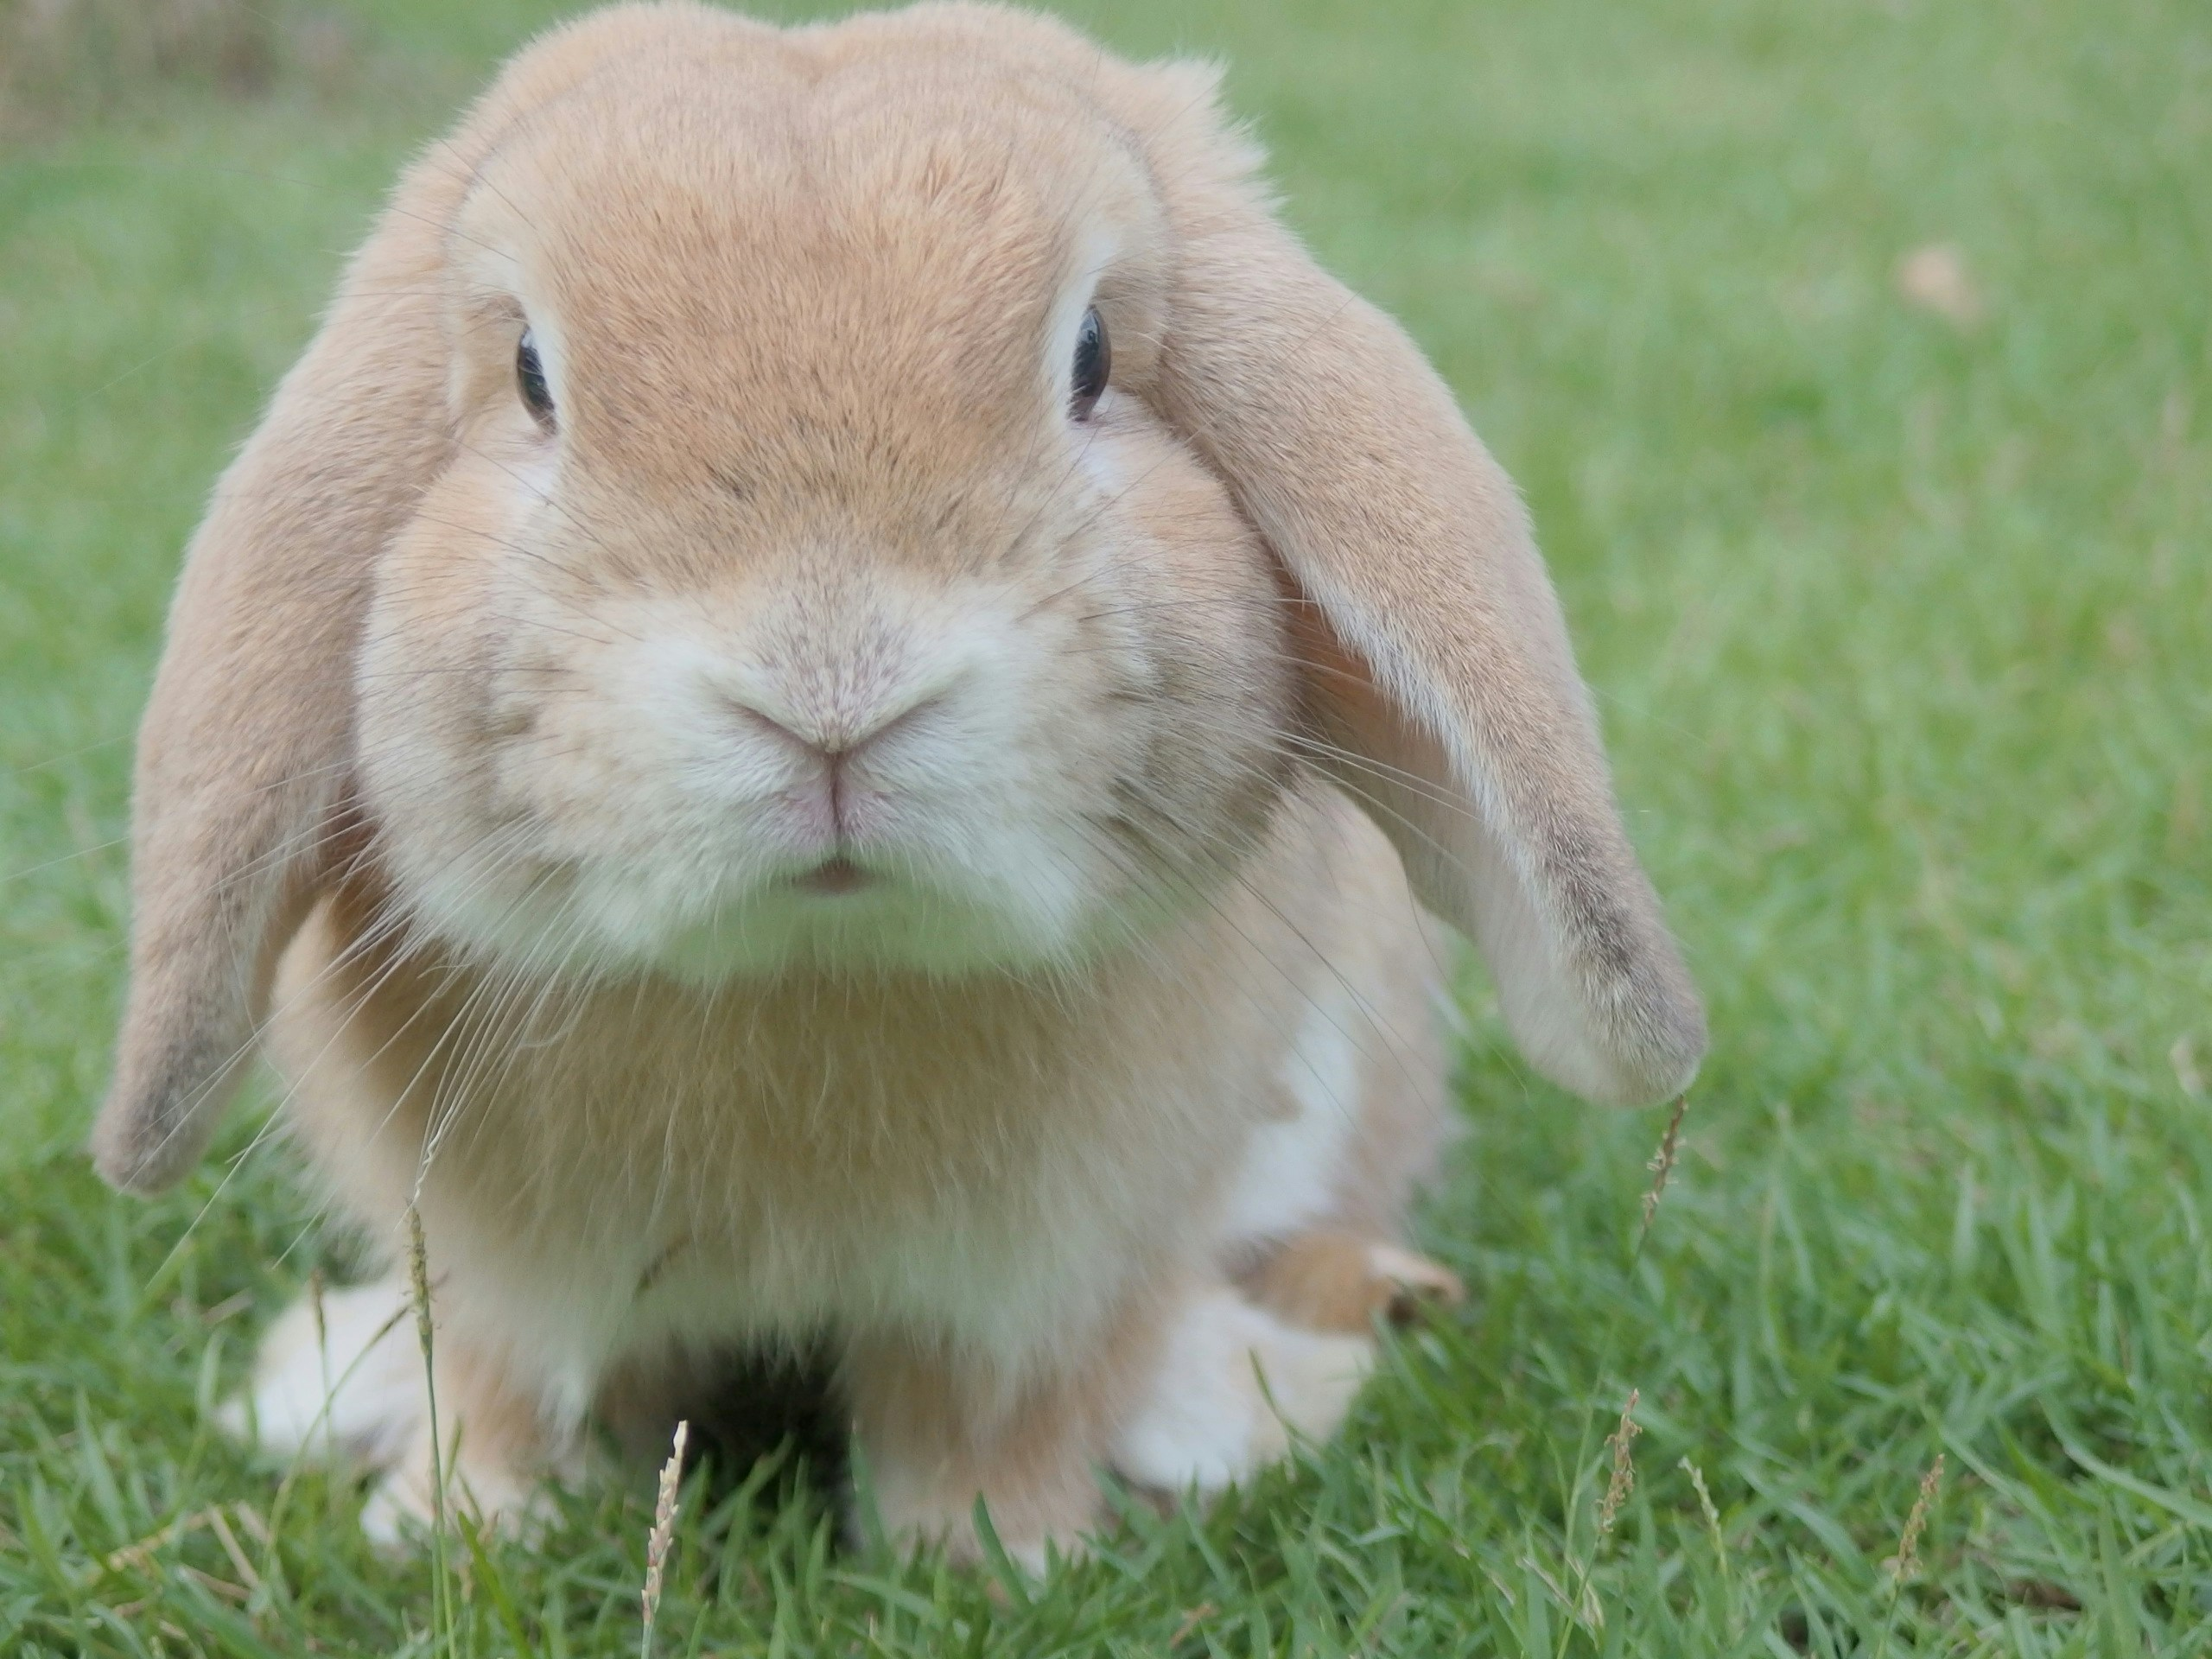
\includegraphics[width=.6\linewidth,right,padding=-.2cm .2cm 0cm .2cm]{graphics/bunny-looking-at-camera.jpg}
      \par
      \includegraphics[width=1.1\linewidth,right]{graphics/coffe-barista-next-to-roaster.jpg}
    \end{column}

    \begin{column}{.40\linewidth}
      %Most cryptographic applications today are susceptible against attacks from quantum computers.

      %\vfil
      %There is no fundamental reason for this – post-quantum cryptography can do many things pre-quantum crypto can do.

      In the following slides you will learn …
      \par\vspace{1.5em}
      … that, to a crypto protocol designer, post-quantum cryptography is not much more than a subtle difference in function interface.
    \end{column}
  \end{columns}
\end{frame}

\begin{frame}[T]{Glossary: Post-Quantum Security}
\small
  \begin{columns}[t,fullwidth]
   \hfill
    \begin{column}{.30\linewidth}
      \begin{block}{Pre-quantum cryptography is …}

      … susceptible to attacks from quantum computers.

\bigskip
      \begin{itemize}
        \item specifically, to\\\emph{Shor's Algorithm} % TODO(karolin): Citation needed
        \item quite fast
        %\item Widely used
        \item widely trusted
      \end{itemize}
      \end{block}
    \end{column}
    \begin{column}{.3\linewidth}
      \begin{block}{Post-quantum cryptography is …}

        … not susceptible to attacks from quantum computers.

\bigskip
      \begin{itemize}
        \item generally less efficient.
        \item much bigger ciphertexts.
        %\item hard to use on embedded devices.
        %\item adoped in the last decade.
        \item less analyzed.
      \end{itemize}
      \end{block}
    \end{column}
    \begin{column}{.3\linewidth}
      \begin{block}{Hybrid cryptography combines …}
        … the combination of the previous two. It is …

\bigskip
        \begin{itemize}
          \item about as inefficient as post-quantum cryptography.
          \item not widely adopted, which is a major problem.
        \end{itemize}
      \end{block}
    \end{column}
    \hfill
  \end{columns}
\end{frame}





\begin{frame}{What Post-Quantum got}
  \includegraphics[width=\linewidth,page=1,clip=true,trim=39 314 39 85]{rosenpass-key-exchanges-nike-kem}
\end{frame}



\begin{frame}[fragile,T]{KEMs and NIKEs}
\small
  \begin{columns}[t,fullwidth]
\hfill
    \begin{column}{.47\linewidth}
\begin{rustblock}{Key Encapsulation Method}
fn Kem::encaps(Pk) -> (Shk, Ct);
fn Kem::decaps(Pk, Ct) -> Shk;

(shk, ct) = encaps(pk);
assert!(decaps(sk, ct) = shk)
\end{rustblock}
\end{column}
\begin{column}{.47\linewidth}
\begin{rustblock}{Non-Interactive Key Exchange}
fn nike(sk: Sk, pk: Pk) -> Shk;

assert!(nike(sk1, pk2) =
        nike(sk2, pk1));
\end{rustblock}
\end{column}\hfill
\end{columns}
\begin{columns}[t,fullwidth]
\hfill
\begin{column}{.47\linewidth}
  Think of it as encrypting a key and sending it
        to the partner.

        \begin{itemize}
          \item secrecy
          \item implicit authentication of recipient
            (assuming they have the shared key, they must
            also have their secret key)
        \end{itemize}
\end{column}
\begin{column}{.47\linewidth}
        Aka. Diffie-Hellman. Note how the
        keypairs are \emph{crossing over} to each other.

        \begin{itemize}
          \item secrecy
          \item implicit mutual authentication
            (for each party: assuming they have the shared key, they must
            also have their secret key)
        \end{itemize}
    \end{column}
    \hfill\strut
  \end{columns}
\end{frame}


\begin{frame}[T,s]{Protocol Security Properties}
  \small
  \begin{columns}[t,fullwidth]
  \hfill
    \begin{column}{.45\linewidth}
      \begin{block}{Implicit authentication}
        \say{If you have access to this shared symmetric key then you must have a particular asymmetric secret key.}
      \end{block}
    \end{column}
    \hfill
    \begin{column}{.45\linewidth}
      \begin{block}{Explicit authentication}
        \say{I know you have access to this shared key because I checked by making you use it, therefore you also have a particular asymmetric secret key.}
      \end{block}
    \end{column}
    \hfill
  \end{columns}

	\bigskip
  \begin{columns}[t,fullwidth]
  \hfill
    \begin{column}{.45\linewidth}
      \begin{block}{Secrecy}
        \say{The data we exchange cannot be decrypted unless someone gets their hands on some of our static keys!}
      \end{block}
    \end{column}
    \hfill
    \begin{column}{.45\linewidth}
      \begin{block}{Forward secrecy}
       \say{Even if our static keys are exposed, the data we exchanged cannot be retroactively decrypted!} *
      \end{block}
    \end{column}
    \hfill
  \end{columns}

  \vspace{1.5em}
  \footnotesize
  * Terms and conditions apply: We are using an extra key that we do not call a \emph{static} key. This key is generated on the fly,
  not written to disk and immediately erased after use, so it is more secure than our static keys. Engaging in cryptography is a magical
  experience but technological constructs can – at best – be asymptotically indistinguishable from miracles.

\end{frame}



\begin{frame}[fragile,T]{KEMs and NIKEs: Key Exchange}
  \begin{columns}[t,fullwidth]
  \hfill
    \begin{column}{.48\linewidth}
      \begin{block}{Key Encapsulation Method}
        \begin{description}[]
          \item[\textbf{Responder Authentication}:] Initiator encapsulates key under the responder public key.
          \item[\textbf{Initiator Authentication}:] Responder encapsulates key under the initiator public key.
          \item[\textbf{Forward Secrecy}:] In case the secret keys get stolen, either party generates a temporary keypair
            and has the other party encapsulate a secret under that keypair.

          \bigskip
          \item[How to do this properly?] See Rosenpass. % TODO: Cite
        \end{description}
      \end{block}
    \end{column}
\hfill
    \begin{column}{.48\linewidth}
      \begin{block}{Non-Interactive Key Exchange}
        \begin{description}[]
          \item[\textbf{Responder Authentication}:] Static-static NIKE since NIKE gives mutual authentication.
          \item[\textbf{Initiator Authentication}:] Static-static NIKE since NIKE gives mutual authentication.
          \item[\textbf{Forward secrecy}:] Another NIKE, involving a temporary keypair.

		\bigskip
          \item[How to do this properly?] See the Noise Protocol Framework. % TODO: Cite
        \end{description}
      \end{block}
    \end{column}\hfill\strut
  \end{columns}
\end{frame}




\begin{frame}[fragile,T]{KEMs and NIKEs}
  \begin{columns}[t,fullwidth]
      \hfill
    \begin{column}{.48\linewidth}
\begin{rustblock}{Key Encapsulation Method}
trait Kem {
  // Secret, Public, Symmetric, Ciphertext
  type Sk; type Pk; type Shk; type Ct;
  fn genkey() -> (Sk, Pk);
  fn encaps(pk: Pk) -> (Shk, Ct);
  fn decaps(sk: Pk, ct: Ct) -> Shk;
}
#[test]
fn test<K: Kem>() {
  let (sk, pk) = K::genkey();
  let (shk1, ct) = K::encaps(pk);
  let shk2 = K::decaps(sk, ct);
  assert_eq!(shk1, shk2);
}
\end{rustblock}
    \end{column}
    \begin{column}{.48\linewidth}
\begin{rustblock}{Non-Interactive Key Exchange}
trait Nike {
  // Secret, Public, Symmetric
  type Sk; type Pk; type Shk;
  fn genkey() -> (Sk, Pk);
  fn nike(sk: Sk, pk: Pk) -> Shk;
}
#[test]
fn test<N: Nike>() {
  let (sk1, pk1) = N::genkey();
  let (sk2, pk2) = N::genkey();
  let ct1 = N::nike(sk1, pk2);
  let ct2 = N::nike(sk2, pk1);
  assert_eq!(ct1, ct2);
}
\end{rustblock}
    \end{column}
	\hfill
  \end{columns}
\end{frame}

\begin{frame}{Rosenpass Key Exchange Parts}
  \centering
  \includegraphics[height=0.91\textheight,page=6,clip=true,trim=40 189 41 74]{rosenpass-key-exchanges-nike-kem}
\end{frame}


% \begin{frame}{Rosenpass Unified Key Exchange}
%   \centering
%   \begin{columns}[fullwidth,c]
%     \begin{column}{.6\linewidth}
%       \includegraphics[width=1.3\linewidth,page=7,clip=true,trim=1cm 4cm 0cm 2cm]{graphics/rosenpass-key-exchanges-nike-kem.pdf}
%     \end{column}%

%     \begin{column}{.4\linewidth}
%       \includegraphics[width=\linewidth,page=5,clip=true,trim=3cm 7cm 0cm 3.5cm]{graphics/rosenpass-key-exchanges-nike-kem.pdf}
%     \end{column}
%   \end{columns}
% \end{frame}





\begin{frame}{Rosenpass Protocol Features}
  \begin{columns}[fullwidth,c]
    \begin{column}{.6\linewidth}
      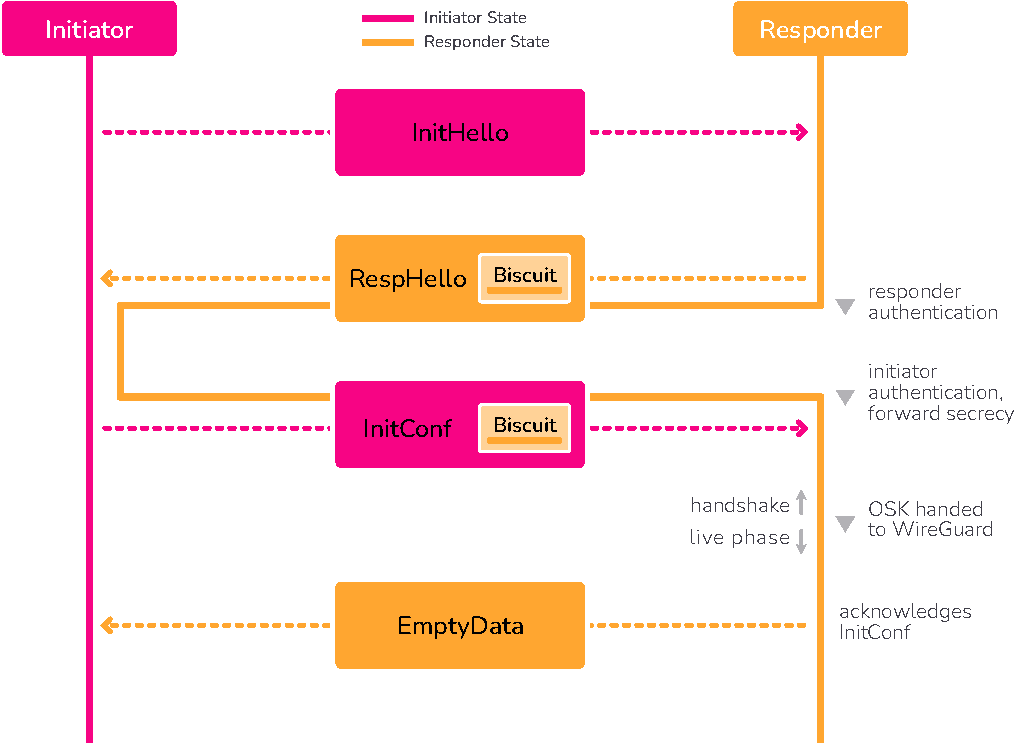
\includegraphics[width=\linewidth]{graphics/rosenpass-wp-key-exchange-protocol-rgb.pdf}
    \end{column}

    \begin{column}{.4\linewidth}
      \begin{itemize}
        \item authenticated key exchange
        \item three KEM operations interleaved to achieve mutual authentication and forward secrecy
        \item no use of signatures
        \item first package (InitHello) is unauthenticated
        \item stateless responder to avoid disruption attacks
      \end{itemize}
    \end{column}
  \end{columns}
\end{frame}
